\documentclass[12pt]{article}
\usepackage[spanish]{babel}
\usepackage{natbib}
\usepackage{url}
\usepackage[utf8x]{inputenc}
\usepackage{amsmath}
\usepackage{float}
\usepackage{subfig}
\usepackage{graphicx}
\graphicspath{{images/}}
\usepackage{parskip}
\usepackage{fancyhdr}
\usepackage{vmargin}
\usepackage{mathtools}
\usepackage{amssymb} 



\title{Actividad \#11:Apocalipsis Zombie}							
\author{\Large Jesùs Valenzuela Nieblas\\}											
\date{\today} 

\makeatletter
\let\thetitle\@title
\let\theauthor\@author
\let\thedate\@date										
\makeatother

\pagestyle{fancy}

\lhead{\thetitle}
\cfoot{\thepage}
\rhead{}
\begin{document}

%%%%%%%%%%%%%%%%%%%%%%%%%%%%%%%%%%%%%%%%%%%%%%%%%%%%%%%%%%%%%%%%%%%%%%%%%%%%%%%%%%%%%%%%%

\begin{titlepage}
	\centering
    \vspace*{.5cm}
     
\includegraphics[scale = 0.7]{logo}\\	% University Logo
    \textsc{\Large Universidad de Sonora}\\[1.0 cm]	% University Name
	\textsc{\Large División de Ciencias Exactas y Naturales}\\[.50 cm]
  	\textsc{\Large Licenciatura en Fìsica}\\[.5 cm]
  \textsc{\large Fìsica Computacional 1}\\[1.5 cm]				% Course Name
	
	{ \huge \bfseries \thetitle}\\

    \vspace*{3 cm}
	\begin{minipage}{\textwidth}
    \centering
    \theauthor
	\end{minipage}\\[3 cm]
	
 
	\vfill
	
\end{titlepage}

%%%%%%%%%%%%%%%%%%%%%%%%%%%%%%%%%%%%%%%%%%%%%%%%%%%%%%%%%%%%%%%%%%%%%%%%%%%%%%%%%%%%%%%%%

\section{Introducciòn}
Un zombi (en ocasiones escrito con la grafía inglesa zombie) es la representación de un cadáver que de una u otra manera puede resucitar o volver a la vida. Muchas de las diferentes relaciones que se muestran con uno de ellos es una figura legendaria propia del culto vudú. Se trata de un muerto resucitado por medios mágicos por un hechicero para convertirlo en su esclavo. De acuerdo con la creencia, un houngan, bokor o hechicero vudú, sería capaz, mediante un ritual, de resucitar a un muerto, que quedaría, sin embargo, sometido en adelante a la voluntad de la persona que le devuelve la vida. También, según una creencia popular, se dice que una persona que es mordida por un zombi, se convierte en zombi.
\begin{figure}[H]
\centering

\includegraphics[scale=.2]{zombie}
\end{figure}
\section{Actividad}

El còdigo utilizado es el siguiente:
\begin{verbatim}

# coding: utf-8

# In[1]:

#MODELO BASICO
import numpy as np
import matplotlib.pyplot as plt
from scipy.integrate import odeint



P = 0.000      # Nacimientos
d = 0.0001     # Muertes 
B = 0.0095     # Infeccion 
G = 0.0001     # Resurreccion 
A = 0.0005     # Destruccion 


def f(y, t):
    Si = y[0]
    Zi = y[1]
    Ri = y[2]
    
    #SED
    f0 = P - B*Si*Zi - d*Si
    f1 = B*Si*Zi + G*Ri - A*Si*Zi
    f2 = d*Si + A*Si*Zi - G*Ri
    return [f0, f1, f2]

# CONDICIONES INICIALES
S0 = 500.                   # Poblacion S inicial
Z0 = 0                      # Poblacion Z inicial
R0 = 10                     # Poblacion R inicial
y0 = [S0, Z0, R0]           # vector de condiciones iniciales

t  = np.linspace(0, 6., 1000)       

# Sol ED
soln = odeint(f, y0, t)
S = soln[:, 0]
Z = soln[:, 1]
R = soln[:, 2]

# Grafica
plt.figure()
plt.ylim(0,500)
plt.grid(True)
plt.plot(t, S,'go', label='Vivos')
plt.plot(t, Z, 'ro',label='Zombies')
plt.xlabel('Tiempo/dias')
plt.ylabel('Poblacion')
plt.title('Modelo Basico')
plt.legend(loc="best")

fig = matplotlib.pyplot.gcf()
fig.set_size_inches(10.5,5.5)
fig.savefig('basico.png',dpi=100)



# In[ ]:

#MODELO LATENTE
import numpy as np
import matplotlib.pyplot as plt
from scipy.integrate import odeint

Pi = 0         # Nacimientos 
Del = 0.0001   # Muertes Naturales 
Bet = 0.0095   # Transmision     
Zet = 0.0001   # Removidos         
Alf = 0.0001   # Destruidos        
Rho = 0.05     # Infecciones        

#SED
def f(y, t):
    Si = y[0]
    Zi = y[1]
    Ri = y[2]
    Ii = y[3]
# Modelo
    f0 = Pi - Bet*Si*Zi - Del*Si                #Si
    f1 = Rho*Ii + Zet*Ri - Alf*Si*Zi            #Zi
    f2 = Del*Si + Del*Ii + Alf*Si*Zi - Zet*Ri   #Ri
    f3 = Bet*Si*Zi -Rho*Ii - Del*Ii             #Ii
    
    return [f0, f1, f2, f3]

S0 = 500.                        # Poblacion Inicial
Z0 = 0.                          # Zombie Inicial
R0 = 0.                          # Muertos Inicial
I0 = 1.                          # Infectados Inicial
y0 = [S0, Z0, R0, I0]            # Condiciones Iniciales
t  = np.linspace(0., 30., 1000)  # Tiempo

# Sol ED
soln = odeint(f, y0, t)
S = soln[:, 0]
Z = soln[:, 1]
R = soln[:, 2]
I = soln[:, 3]
# Grafica
plt.figure()
plt.ylim(0,500)
plt.grid(True)
plt.plot(t, S,'ro' ,label='Vivos')
plt.plot(t, Z, 'yo',label='Zombies')
plt.xlabel('Tiempo/dias')
plt.ylabel('Poblacion')
plt.title('Modelo Latente.')
plt.legend(loc="best")


fig = matplotlib.pyplot.gcf()
fig.set_size_inches(10.5,5.5)
fig.savefig('latente.png',dpi=100)


# In[ ]:

#MODELO CON CUARENTENA
import numpy as np
import matplotlib.pyplot as plt
from scipy.integrate import odeint

Pi = 0         # Nacimientos Diarios
Del = 0.0001   # Muertes Naturales 
Bet = 0.0095   # Transmision       
Zet = 0.0001   # Removidos        
Alf = 0.0001   # Destruidos        
Rho = 0.05     # Infected          
Kap = 0.15     # Infectados Q      
Sig = 0.10     # Infected         
Gam = 0.001    # Infected          

#SED
def f(y, t):
    Si = y[0]
    Zi = y[1]
    Ri = y[2]
    Ii = y[3]
    Qi = y[4]
    # Modelo
    f0 = Pi - Bet*Si*Zi - Del*Si                        #Si
    f1 = Rho*Ii + Zet*Ri - Alf*Si*Zi - Sig*Zi           #Zi
    f2 = Del*Si + Del*Ii + Alf*Si*Zi - Zet*Ri + Gam*Qi  #Ri
    f3 = Bet*Si*Zi -Rho*Ii - Del*Ii - Kap*Ii            #Ii
    f4 = Kap*Ii + Sig*Zi - Gam*Qi                       #Qi
    return [f0, f1, f2, f3, f4]

S0 = 500                        # Poblacion Inicial
Z0 = 0                          # Zombie Inicial
R0 = 0                          # Muertos Inicial
I0 = 1                          # Infectados Inicial
Q0 = 0                          # Cuarentena Inicial
y0 = [S0, Z0, R0, I0, Q0]       # Condiciones Iniciales
t  = np.linspace(0., 30., 1000) # Tiempo

# Sol ED
soln = odeint(f, y0, t)
S = soln[:, 0]
Z = soln[:, 1]
R = soln[:, 2]
I = soln[:, 3]
Q = soln[:, 4]
# Grafica
plt.figure()
plt.ylim(0,500)
plt.grid(True)
plt.plot(t, S,'go', label='Vivos')
plt.plot(t, Z,'yo', label='Zombies')
plt.xlabel('Tiempo/dias')
plt.ylabel('Poblacion')
plt.title('Modelo con Caurentena.')
plt.legend(loc="best")

fig = matplotlib.pyplot.gcf()
fig.set_size_inches(10.5,5.5)
fig.savefig('cuarentena.png',dpi=100)


# In[ ]:

#MODELO CON TRATAMIENTO
import numpy as np
import matplotlib.pyplot as plt
from scipy.integrate import odeint


Pi  = 0        # Nacimientos Diarios
Del = 0.0001   # Muertes Naturales 
Bet = 0.0095   # Transmisiones   
Zet = 0.0001   # Removidos      
Alf = 0.0001   # Destruidos       
Rho = 0.05     # Infectados          
Ce  = 0.05     # Cura   

#SED
def f(y, t):
    Si = y[0]
    Zi = y[1]
    Ri = y[2]
    Ii = y[3]
    # Modelo
    f0 = Pi - Bet*Si*Zi - Del*Si +Ce*Zi             #Si
    f1 = Rho*Ii + Zet*Ri - Alf*Si*Zi -Ce*Zi         #Zi
    f2 = Del*Si + Del*Ii + Alf*Si*Zi - Zet*Ri       #Ri
    f3 = Bet*Si*Zi -Rho*Ii - Del*Ii                 #Ii
    
    return [f0, f1, f2, f3]

S0 = 500                        # Poblacion Inicial
Z0 = 0                          # Zombie Inicial
R0 = 0                          # Muertos Inicial
I0 = 1                          # Infectados Inicial
y0 = [S0, Z0, R0, I0]           # Condiciones Iniciales
t  = np.linspace(0., 30., 1000) # Tiempo

# Solucion E.D.
soln = odeint(f, y0, t)
S = soln[:, 0]
Z = soln[:, 1]
R = soln[:, 2]
I = soln[:, 3]
# Grafica
plt.figure()
plt.ylim(0,500)
plt.grid(True)
plt.plot(t, S,'go', label='Vivos')
plt.plot(t, Z,'ro', label='Zombies')
plt.xlabel('Tiempo/dias')
plt.ylabel('Poblacion')
plt.title(' Modelo con Tratamiento')
plt.legend(loc="best")

fig = matplotlib.pyplot.gcf()
fig.set_size_inches(10.5,5.5)
fig.savefig('tratamiento.png',dpi=100)


# In[ ]:

#MODELO CON ERRADICACION
import numpy as np
import matplotlib.pyplot as plt
from scipy.integrate import odeint


Pi  = 0        # Nacimientos Diarios
Del = 0.0001   # Muertes Naturales
Bet = 0.0055   # Transmision       
Zet = 0.0900   # Removidos         
Alf = 0.0075   # Destruidos        
k = 0.25
n=4

# solve the system dy/dt = f(y, t)
def f(y, t):
    Si = y[0]
    Zi = y[1]
    Ri = y[2]
    # Modelo
    f0 = Pi - Bet*Si*Zi - Del*Si                  
    f1 = Bet*Si*Zi + Zet*Ri - Alf*Si*Zi          
    f2 = Del*Si + Alf*Si*Zi - Zet*Ri              
    f3 = -k*n*Zi                                  
    
    return [f0, f1, f2, f3]

# CI
S0 = 500                        # Poblacion Inicial
Z0 = 0                          # Zombie Inicial
R0 = 0                          # Muertos Inicial
DZ0 = 0                         # Infectados Inicial
y0 = [S0, Z0, R0, DZ0]           # Condiciones Iniciales
t  = np.linspace(0., 130., 1000) # Tiempo

# Sol ED
soln = odeint(f, y0, t)
S = soln[:, 0]
Z = soln[:, 1]
R = soln[:, 2]
I = soln[:, 3]

# Grafica
plt.figure()
plt.ylim(0,500)
plt.grid(True)
plt.plot(t, S,'go', label='Vivos')
plt.plot(t, Z,'yo',label='Zombies')
plt.xlabel('Tiempo/dias')
plt.ylabel('Poblacion')
plt.title('Modelo con Erradicacion Impulsiva')
plt.legend(loc="best")


fig = matplotlib.pyplot.gcf()
fig.set_size_inches(10.5,5.5)
fig.savefig('erradicacion.png',dpi=100)


\end{verbatim}
\section{Gráficas}
\subsection{Modelo Basico}
\begin{figure}[H]
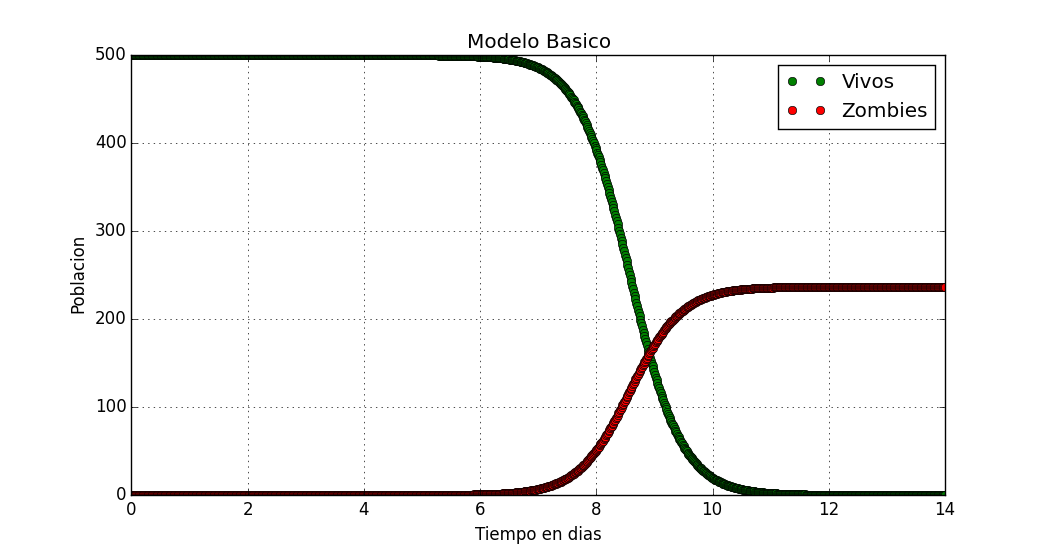
\includegraphics[scale=.6]{basico}
\end{figure}
\subsection{Modelo Latente}
\begin{figure}[H]
\includegraphics[scale=.6]{latente}
\end{figure}\subsection{Modelo en cuarentena}
\begin{figure}[H]
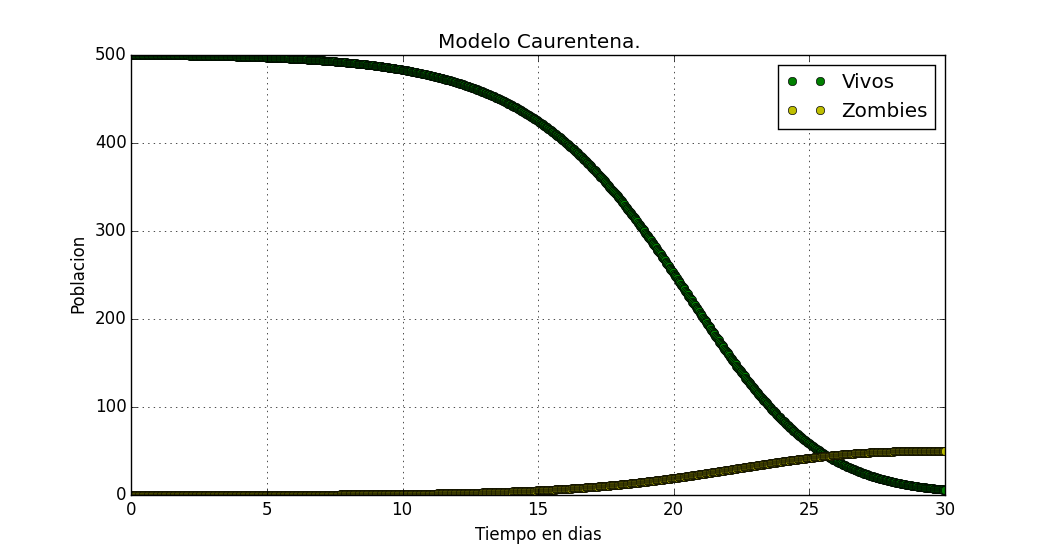
\includegraphics[scale=.6]{cuarentena}
\end{figure}\subsection{Modelo en tratamiento}
\begin{figure}[H]
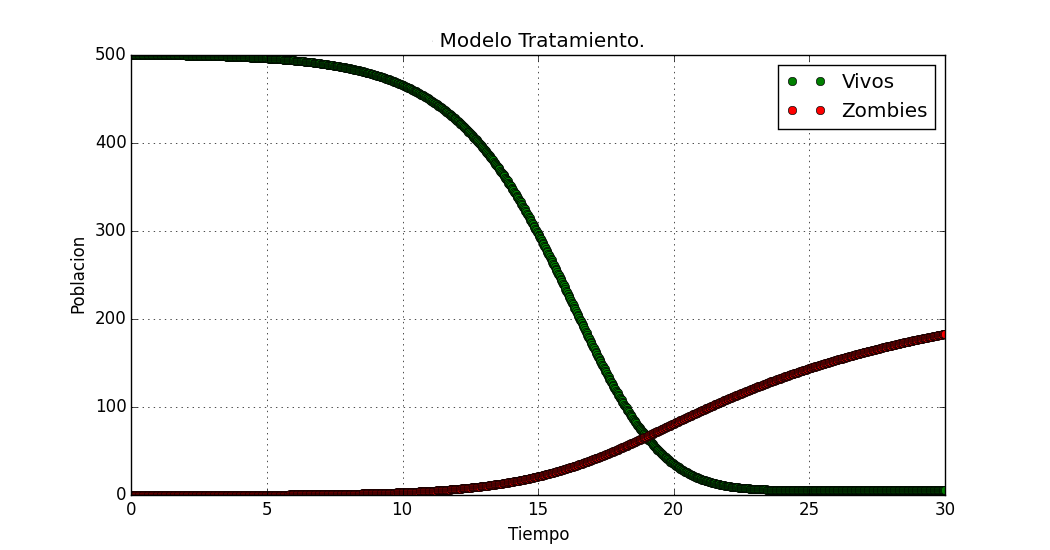
\includegraphics[scale=.6]{tratamiento}
\end{figure}\subsection{Modelo con erradicacion impulsiva}
\begin{figure}[H]
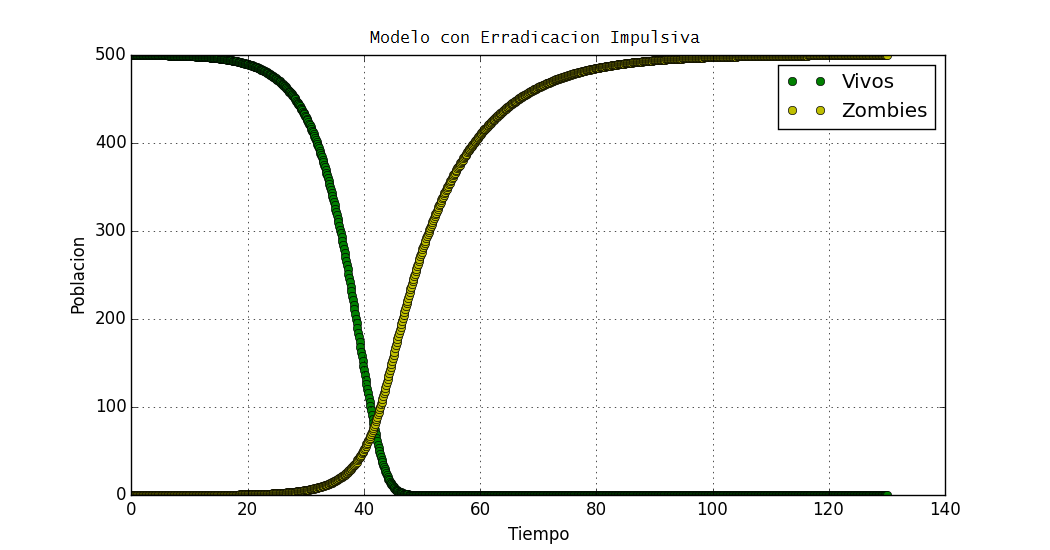
\includegraphics[scale=.6]{erradicacion}
\end{figure}


\end{document}
